\documentclass[../../e3_tp3_main.tex]{subfiles}

\begin{document}

%capítulo
\chapter{Ejercicio 3}

The input of the system is $W$ and the output is $Z$. $Z=1$ if there has just been a transition from 0 to 1, and $Z=0$ otherwise. 

\section{Moore-type FSM implementation}
\subsection{FSM flow-chart}
\begin{equation}
	\tikzfig{moore_machine}
\end{equation}

\subsection{State descriptions}
\begin{table}[H]	%mealy state descriptions
	\centering
	\begin{tabular}{|c|c|}
	\hline	
	$y_0$, $y_1$  & Description\\	
	\hline 
	00 & The last number detected is a 0\\ 
	\hline 
	01 & The last two numbers detected were 0-1 (in order).\\ 
	\hline 
	10 & The last two numbers detected were 1-1.\\ 
	\hline
	
	\end{tabular} 
	\caption{Possible states for the Mealy-type FSM implementation.}
	\label{tab:ej3_moore_states}
\end{table}


\subsection{State transition table}
\begin{table}[H]	%moore state transition table
	\centering
		\begin{tabular}{|c|c|c|c|}
		\hline 
		state\textbackslash W & 0 & 1 & output\\ 
		\hline 
		00 & 00 & 01 & 0\\ 
		\hline 
		01 & 00 & 10 & 1\\ 
		\hline 
		10 & 00 & 10 & 0\\ 
		\hline 
		\end{tabular} 
	\caption[States transitions and outputs for the Moore-type FSM implementation]{States transitions and outputs for the Moore-type FSM implementation. Each cell indicates the next state}
	\label{tab:ej3_moore_transitions}
\end{table}

\subsection{Outputs and next states Karnaugh maps}

\begin{figure}[H]
	\centering
	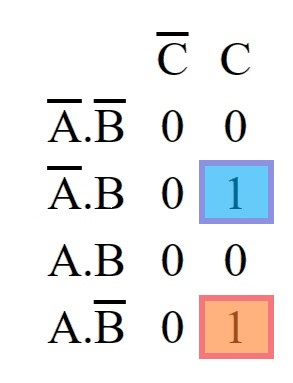
\includegraphics[scale=1]{figures/e3_tp3_ej3_moore_y0_kmap.jpg}
	\caption{$Y_0$ Karnaugh map}
\end{figure}

\begin{figure}[H]
	\centering
	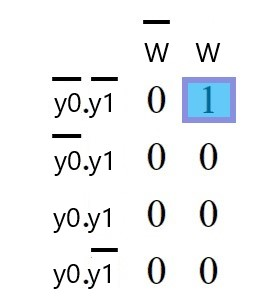
\includegraphics[scale=1]{figures/e3_tp3_ej3_moore_y1_kmap.jpg}
	\caption{$Y_1$ Karnaugh map}
\end{figure}

\begin{figure}[H]
	\centering
	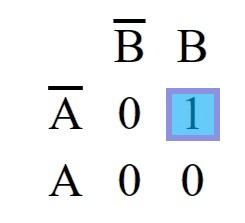
\includegraphics[scale=0.9]{figures/e3_tp3_ej3_moore_z_kmap.jpg}
	\caption{$Z$ Karnaugh map}
\end{figure}

\subsection{Outputs and next states schematics}
%schematics as sum-of-products


\section{Mealy-type FSM implementation}
\subsection{FSM flow-chart}
\begin{equation}
	\tikzfig{mealy_machine}
\end{equation}

The system can be implemented with a Mealy-type FSM with 2 states (see table \ref{tab:ej3_mealy_states}).

\subsection{State descriptions}
\begin{table}[H]	%mealy state descriptions
	\centering
	\begin{tabular}{|c|c|}
	\hline	
	$y_0$  & Description\\	
	\hline 
	0 & The last number detected is a 0\\ 
	\hline 
	1 & The last number detected is a 1\\ 
	\hline 

	\end{tabular} 
	\caption{Possible states for the Mealy-type FSM implementation.}
	\label{tab:ej3_mealy_states}
\end{table}


\subsection{State transition table}
\begin{table}[H]
	\centering
	\begin{tabular}{|c|c|c|}
		\hline 
		state\textbackslash W & 0 & 1 \\ 
		\hline 
		0 & 0/0 & 1/1 \\ 
		\hline 
		1 & 0/0 & 1/0 \\ 
		\hline 
	\end{tabular} 
	\caption[States transitions and outputs for the Mealy-type FSM implementation]{States transitions and outputs for the Mealy-type FSM implementation. Each cell has the format $next\, state\, / \, Z$}
	\label{tab:ej3_mealy_transitions}
\end{table}

The state transition and outputs are shown in table \ref{tab:ej3_mealy_transitions}. This can be separated in two other tables which correspond to the values of $Y_0$ and $Z$ for every combination of $y_0$ and $W$. Then, the minimal sum-of-products expressions for these variables are obtained. 

\subsection{Outputs and next states Karnaugh maps}

\begin{figure}[H]
	\centering
	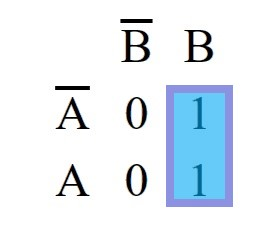
\includegraphics[scale=1]{figures/e3_tp3_ej3_mealy_y0_kmap.jpg}
	\caption{$Y_0$ Karnaugh map}
\end{figure}

\begin{figure}[H]
	\centering
	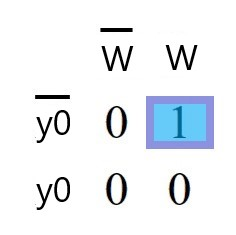
\includegraphics[scale=1]{figures/e3_tp3_ej3_mealy_z_kmap.jpg}
	\caption{$Z$ Karnaugh map}
\end{figure}


\subsection{Output and next states schematics}
%schematics as sum-of-products


\end{document}
